\documentclass[a4paper,12pt]{report}

\usepackage{cmap}
\usepackage[T2A]{fontenc}
\usepackage[utf8]{inputenc}
\usepackage[english,russian]{babel}
\usepackage{listings}
\usepackage{amsmath}
\usepackage{amsfonts}
\usepackage{float}
\usepackage{csquotes}
\usepackage{hyphenat}

% \usepackage{titlesec}
% \newcommand{\sectionbreak}{\clearpage}

\usepackage{graphicx}
\graphicspath{ {./images/} }

\usepackage{xcolor}
% \usepackage{courier}

\usepackage[
    backend=biber,
    style=alphabetic,
    sorting=ynt
]{biblatex}
\addbibresource{resources.bib}

\definecolor{buzzlightyear}{HTML}{8757A5}
\definecolor{grass}{HTML}{738D06}
\definecolor{sand}{HTML}{F18A2B}
\definecolor{comment}{HTML}{8E908B}

\lstdefinestyle{habrstyle}{
    backgroundcolor=\color{white},   
    commentstyle=\color{comment},
    keywordstyle=\bfseries\color{buzzlightyear},
    numberstyle=\tiny\color{comment},
    stringstyle=\color{grass},
    basicstyle=\ttfamily\footnotesize,
    breakatwhitespace=false,         
    breaklines=true,                 
    captionpos=b,                    
    keepspaces=true,                 
    numbers=left,                    
    numbersep=5pt,                  
    showspaces=false,                
    showstringspaces=false,
    showtabs=false,                  
    tabsize=4
}

\lstset{style=habrstyle}

\author{Луняк Николай}
\title{Лабораторная работа 10}
\date{\today}

\begin{document}
    \maketitle
    \tableofcontents
    \listoffigures
    \lstlistoflistings
    
    \chapter{Импорты}
    
    \textquote{Полезные штуки} на все случаи жизни.
    
\begin{lstlisting}[language=Python,caption=Импорты]
from thinkdsp import Signal, Sinusoid, SquareSignal, TriangleSignal, SawtoothSignal, ParabolicSignal
from thinkdsp import normalize, unbias, PI2, decorate
from thinkdsp import Chirp
from thinkdsp import read_wave
from thinkdsp import Spectrum, Wave, UncorrelatedGaussianNoise, Spectrogram
from thinkdsp import Noise
from thinkdsp import CubicSignal
from thinkdsp import zero_pad

import numpy as np
import pandas as pd

from matplotlib import pyplot as plt

import thinkstats2

from scipy.stats import linregress

import scipy
import scipy.fftpack

import scipy.signal

from ipywidgets import interact, interactive, fixed
import ipywidgets as widgets

loglog = dict(xscale='log', yscale='log')

PI2 = np.pi * 2
\end{lstlisting}

    \chapter{Дополняем нулями}
    
    В разделе 10.4 была рассмотрена операция \emph{линейной} свертки, а в 10.3 выполнялась \emph{циклическая}. \textquote{Превратить} ее в линейную можно было бы при помощи встаки нулей в конец. 
    
    Возьмем уже рассмотренные звуки выстрела и скрипки, обрежем их до $2^16$ и дополним нулями до $2^17$.
    
\begin{lstlisting}[language=Python,caption=Сигнал выстрела]
response = read_wave('Sounds/180960__kleeb__gunshot.wav')

start = 0.12
response = response.segment(start=start)
response.shift(-start)

response.truncate(2**16)
response.zero_pad(2**17)

response.normalize()
response.plot()
decorate(xlabel='Time (s)')
\end{lstlisting}

    \begin{figure}[H]
        \centering
        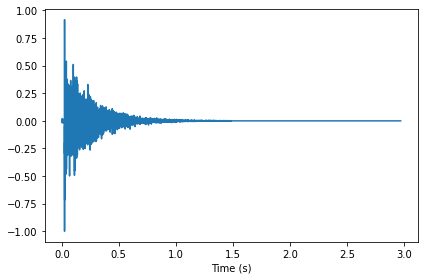
\includegraphics[width=0.75\textwidth]{images/ex1_shot_1.png}
        \caption{Вытрел, дополненный нулями}
        \label{fig:ex1_shot_1}
    \end{figure}
    
    Вот его спектр.
    
\begin{lstlisting}[language=Python,caption=Спектр выстрела]
transfer = response.make_spectrum()
transfer.plot()
decorate(xlabel='Frequency (Hz)', ylabel='Amplitude')
\end{lstlisting}

    \begin{figure}[H]
        \centering
        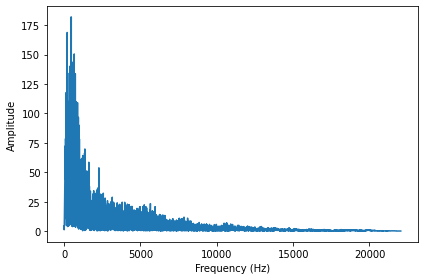
\includegraphics[width=0.75\textwidth]{images/ex1_shot_2.png}
        \caption{Спектр}
        \label{fig:ex1_shot_2}
    \end{figure}
    
    Загружаем скрипку.
    
\begin{lstlisting}[language=Python,caption=Сигнал скрипки]
violin = read_wave('Sounds/92002__jcveliz__violin-origional.wav')

start = 0.11
violin = violin.segment(start=start)
violin.shift(-start)

violin.truncate(2**16)
violin.zero_pad(2**17)

violin.normalize()
violin.plot()
decorate(xlabel='Time (s)')
\end{lstlisting}

    \begin{figure}[H]
        \centering
        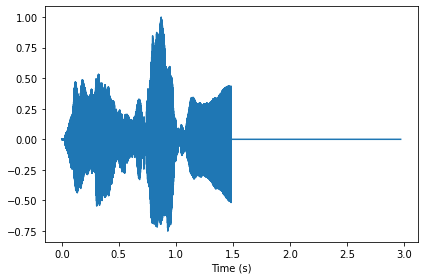
\includegraphics[width=0.75\textwidth]{images/ex1_violin_1.png}
        \caption{Сигнал скрипки с нулями}
        \label{fig:ex1_violin_1}
    \end{figure}
    
    Подействуем спектром передаточной функцией системы на скрипку (содержит свойства комнаты, где был записан выстрел).
    
\begin{lstlisting}[language=Python,caption=Перемножаем спектры]
spectrum = violin.make_spectrum()
output = (spectrum * transfer).make_wave()
output.normalize()
output.plot()
\end{lstlisting}

    \begin{figure}[H]
        \centering
        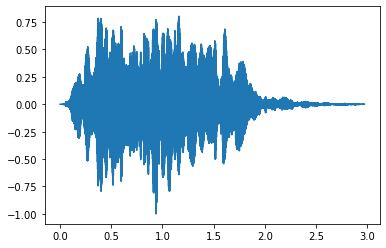
\includegraphics[width=0.75\textwidth]{images/ex1_violin_2.png}
        \caption{Результат воздействия}
        \label{fig:ex1_violin_2}
    \end{figure}
    
    Теперь проделаем то же самое, но при помощи свертки. Сначала уберем нули, которые мы вставили в конец.
    
\begin{lstlisting}[language=Python,caption=Убираем нули в звуке выстрела]
response.truncate(2**16)
response.plot()
\end{lstlisting}

    \begin{figure}[H]
        \centering
        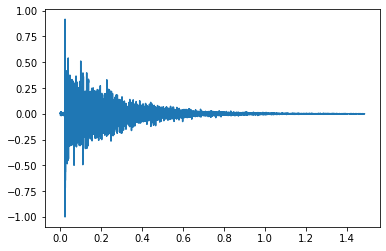
\includegraphics[width=0.75\textwidth]{images/ex1_shot_3.png}
        \caption{Выстрел без дополненительных нулей}
        \label{fig:ex1_shot_3}
    \end{figure}
    
\begin{lstlisting}[language=Python,caption=Убираем нули в звуке скрипки]
violin.truncate(2**16)
violin.plot()
\end{lstlisting}

    \begin{figure}[H]
        \centering
        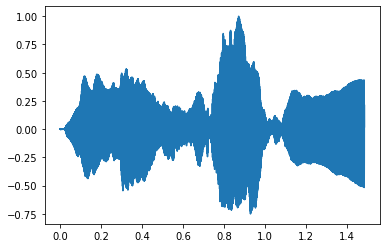
\includegraphics[width=0.75\textwidth]{images/ex1_violin_3.png}
        \caption{Скрипка без дополненительных нулей}
        \label{fig:ex1_violin_3}
    \end{figure}
    
    Выполняем свертку.
    
\begin{lstlisting}[language=Python,caption=Свертка]
output2 = violin.convolve(response)
output2.plot()
\end{lstlisting}

    \begin{figure}[H]
        \centering
        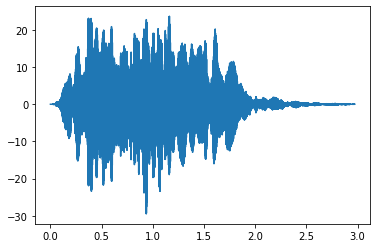
\includegraphics[width=0.75\textwidth]{images/ex1_convolution_1.png}
        \caption{Результат свертки}
        \label{fig:ex1_convolution_1}
    \end{figure}
    
    Разницы в картинках не видно. Если сравнить результат на слух, уловить какую-то разницу тоже не удастся. Единственный нюанс заключается лишь в том, что \sloppy{\texttt{len(output)}} и \sloppy{\texttt{len(output2)}} равны 131072 и 131071 соответственно.

    \chapter{Симулируем какой-нибудь свой звук}
    
    В качестве импульса возьмем это: \sloppy{\texttt{https://www.openair.hosted.york.ac.uk/?page\_id=425}}, а подопытным звуком пусть будет: \sloppy{\texttt{https://freesound.org/people/JarredGibb/sounds/233099/}}.
    
\begin{lstlisting}[language=Python,caption=Загрузка импульса]
response = read_wave('Sounds/s1r2_0_1.wav')

start = 0.08
duration = 1
response = response.segment(start=start, duration=duration)
response.shift(-start)

response.normalize()
response.plot()
decorate(xlabel='Time (s)')
\end{lstlisting}

    \begin{figure}[H]
        \centering
        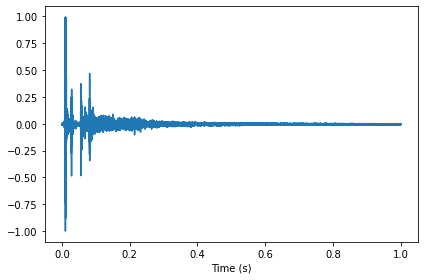
\includegraphics[width=0.75\textwidth]{images/ex2_response_1.png}
        \caption{Импульс}
        \label{fig:ex2_response_1}
    \end{figure}
    
\begin{lstlisting}[language=Python,caption=Спектр импульса]
transfer = response.make_spectrum()
transfer.plot()
decorate(xlabel='Frequency (Hz)', ylabel='Amplitude')
\end{lstlisting}

    \begin{figure}[H]
        \centering
        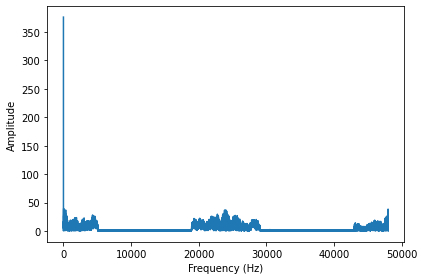
\includegraphics[width=0.75\textwidth]{images/ex2_response_2.png}
        \caption{Спектр}
        \label{fig:ex2_response_2}
    \end{figure}
    
    Теперь возьмем наш второй звук.
    
\begin{lstlisting}[language=Python,caption=Зугрузка кряка]
wave = read_wave('Sounds/233099__jarredgibb__goose-horn-1-96khz.wav')

start = 0.28
wave = wave.segment(start=start)
wave.shift(-start)

wave.truncate(len(response))
wave.normalize()
wave.plot()
decorate(xlabel='Time (s)')
\end{lstlisting}

    \begin{figure}[H]
        \centering
        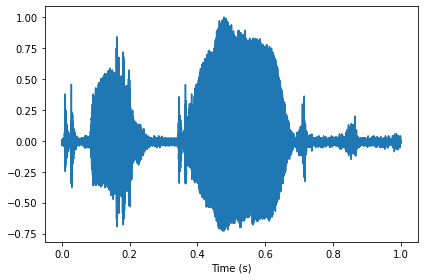
\includegraphics[width=0.75\textwidth]{images/ex2_horn_1.png}
        \caption{Кряк}
        \label{fig:ex2_horn_1}
    \end{figure}
    
    Применим "эффект".
    
\begin{lstlisting}[language=Python,caption=Трансформация]
output = (spectrum * transfer).make_wave()
output.normalize()
output.plot()
\end{lstlisting}

    \begin{figure}[H]
        \centering
        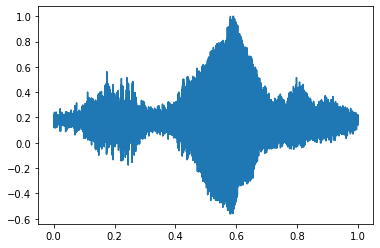
\includegraphics[width=0.75\textwidth]{images/ex2_horn_2.png}
        \caption{Спектр}
        \label{fig:ex2_horn_2}
    \end{figure}
    
    Если прослушать теперь кряк "до" и кряк "после", то кажется, что второй произошел там же, где записывали импульс. Аналогичное решение получаем и через свертку:
    
\begin{lstlisting}[language=Python,caption=Трансформация (х2)]
ys = scipy.signal.fftconvolve(wave.ys, response.ys)
convolved2 = Wave(ys, framerate=wave.framerate)
convolved2.normalize()
convolved2.make_audio()
\end{lstlisting}

    % \printbibliography
    
\end{document}
